%        File: ecologyletters.tex
%     Created: Sat Oct 29 02:00 PM 2011 P
% Last Change: Sat Oct 29 02:00 PM 2011 P
%

% Title page
% - author contributions
%- the article title
%- the full name(s) of all author(s), affiliation(s), e-mail address(es) of all author(s)
%- a short running title (abbreviated form of title) of less than 45 characters including spaces
%- up to 10 keywords for indexing purposes. It is very important that the keywords be chosen carefully.
%- the type of article (Ideas and Perspectives, Letter, or Reviews and Syntheses)
%- the number of words in the abstract, in the manuscript as a whole, and in the main text (excluding abstract, acknowledgements, references, table and figure legends)
%- the number of references (or for papers with extensive meta-analyses, the number of data-source references AND the number of general references)
%- the number of figures and tables
%- the name and complete mailing address (including telephone and fax numbers and e-mail address) of the person to whom correspondence should be sent.
%


%\documentclass[authoryear,5p]{elsarticle}
\documentclass[authoryear,preprint,11pt]{elsarticle}
\bibliographystyle{elsarticle-harv}
\usepackage{graphicx}
\usepackage{amsmath,amsfonts}
\usepackage{lineno}
\linenumbers
\usepackage{subfigure}
\usepackage[pdftex]{color}
\definecolor{darkblue}{rgb}{0,0,0.5}
\definecolor{darkgreen}{rgb}{0,0.5,0}
%\usepackage[pdftex, colorlinks, citecolor=darkblue,linkcolor=darkgreen]{hyperref}
\usepackage[pdftex, colorlinks]{hyperref}
\textwidth 6.75in
\oddsidemargin -0.15in
\evensidemargin -0.15in
\textheight 9in
\topmargin -0.5in
\newcommand{\ud}{\mathrm{d}}
\newcommand{\E}{\mathrm{E}}
\newcommand{\C}{\mathrm{Cov}}
\newcommand{\V}{\mathrm{Var}}

\journal{\tiny Ecology Letters} 
\begin{document}
\begin{frontmatter}
  \title{Quantifying Limits to Detection of Early Warning for Critical Transitions}
  \author[cpb]{Carl Boettiger\corref{cor1}}
  \ead{cboettig@ucdavis.edu, 610-389-6087}
  \author[esp]{Alan Hastings}
  %\author[info]{}
  %\author[davis]{}
  \cortext[cor1]{Corresponding author.}
  \address[cpb]{Center for Population Biology, 1 Shields Avenue, University of California, Davis, CA, 95616 United States.}
  \address[esp]{Department of Environmental Science and Policy, University of California, Davis} 

 % \address[info]{ \\ 
  %              }

  \begin{abstract}

Catastrophic regime shifts in complex natural systems may be averted through advanced detection. 
Recent work has provided a proof-of-principle that many systems approaching a catastrophic transition may be identified 
through the lens of early warning indicators such as rising variance or increased return times.  
Without the benefit of hindsight of a collapse, 
applications of these approaches must quantify how reliable different indicators are in avoiding false alarms, 
and how sensitive they are to missing subtle warning signs.  
We propose an approach which quantifies this trade-off between reliability and sensitivity, 
allows comparisons between different indicators, 
and estimates what data are necessary to achieve a desired error rate. 
We show these error rates can be quite severe for common indicators even under favorable assumptions, 
and illustrate how a likelihood-based indicator can improve this performance.  

  \end{abstract}

  \begin{keyword}
early warning signals \sep tipping point \sep alternative stable states \sep likelihood methods 
   \end{keyword}
 \end{frontmatter}
%\emph{\noindent \textbf{Running title}: Limits to Detection of Early Warning \\ 
%  \textbf{Article Type}: Letter.  Abstract: 132 words, Text: 3,472 words, 34 references, 4 Figures. \\
%  \textbf{Author Contributions}: C.B. wrote the software and performed the analysis with advice from A.H.  C.B. and A.H. designed the study and wrote the paper. 
% }

\section{Introduction}
There is an increasing recognition of the importance of regime shifts or critical transitions at a variety of scales in ecological systems~\citep{Holling1973, Wissel1984, Scheffer2001, Scheffer2009, Drake2010, Carpenter2011}⁠. 
Many important ecosystems may currently be threatened with collapse, including corals~\citep{Bellwood2004}, fisheries~\citep{Berkes2006}⁠, lakes~\citep{Carpenter2011}, and semi-arid ecosystems~\citep{Kefi2007}⁠. 
Given the potential impact of  these shifts on the sustainable delivery of ecosystem services
and the idea that management responses would be needed either to avoid an undesirable shift or else to adapt to novel conditions,
it is important to develop the ability to predict impending regime shifts based on early warning signs. 
With a good model of the system, detail-oriented approaches could be useful~\citep{Lenton2009},
but in cases where specific models are not available general approaches are needed~\citep{Scheffer2009}⁠.

We focus on the common scenario of a gradual environmental change yielding a sudden shift or bifurcation in a system 
(\emph{i.e.} where the dominant eigenvalue passes through zero,
as discussed in~\citet{Scheffer2001, Scheffer2009}). 
Making this assumption provides a ``best-case'' test of detection approaches;
we will demonstrate the resulting uncertainty can be very high.
We describe a novel statistical approach for handling uncertainty that is appropriate for the goal of informing management.  


\subsection{The implicit model}
Foundational work on early warning signals has operated under the often-implicit assumption that the system dynamics contain a saddle-node bifurcation and looks for patterns that would be associated with approaching this bifurcation point.  The typical pattern has been a trend in a summary statistic such as variance, autocorrelation, skew, spectral ratio~\citep{Biggs2009}.  While attractive for their simplicity, such approaches are subject to numerous challenges.

1) While superficially simple, 
calculation of these statistics is subject to 
several somewhat arbitrary decisions and additional assumptions,
such as the choice of window size over which the statistic is computed,
the choice of detrending,
whether the consecutive averaging windows should overlap~\citep[\emph{e.g.}][]{Lenton2012}. % discusses these challenges, as does most of the others to lesser extent 
% ergodic problem

2) The warning signal, ``an increase in statistic $x$,'' is not quantitative,
making it difficult to attribute statistical significance to this statement.
While much of the literature employing these statistics simply avoids 
any attempt to quantify the significance of the detection, 
\citet{Dakos2008} relies on Kendall's correlation coefficient to quantify an increase,
and then goes through some pains to consider potential null models
that could be used to calculate statistical significance.  
Other measures of increase, such as Pearson's, have also been proposed.  

3) Specifying an apprpriate null model for such a calculation is difficult.  
A supposed strength of the summary statistic approach 
the non-parametric significance test for Kendalls' tau tests against the null model that the sequence is independent,
something that is clearly violated when the statistic is computed in a sliding window.
Not surprisingly, \citet{Dakos2008} find this method overestimates the number of significant events relative to other nulls.  
Other non-parametric methods are tempting, 
such as shuffling the order of the data-points in the time-series,
but this breaks even the natural autocorrelation expected in a stable system that is not approaching any transition,
and thus should not be considered for a null.  
Relying on a more explicit but flexible model %or class of models
such as autogregressive processes is more consistent.  
% Does this go here?
We will see that such generic model-based approaches are becoming more common, 
and argue how they can be used to maximum advantage
% by simulation, likelihood fitting, and ROC curves.  

% See Seekell et al for a summary stat with a good null


4) The underlying assumption that the system contains a saddle-node bifurcation
can be easilyoverlooked in summary-statistic based approach.  
For instance, variance may increase for a wide variety of reasons that 
do not signal an approaching transition~\citep{Schreiber2003, Schreiber2008} 
or may not increase as a bifurcation is approached~\citep{Livnia2012, Dakos2011a}.


% Does this section go here?
A system may experience a critical transition due to a rare fluctuation,
or a perturbation to the system state, %(Does this need a figure)?
rather than a bifurcation~\citep{Scheffer2001, Scheffer2009}.  
When applying detection approaches to data that have already experienced a critical transition,
we must condition on the 
and attempting to ascertain the cause of the transition
These are alternative null hypotheses 
 %(Dakos 2008, Lenton,  see Lenton 2009 transition, see 
\citep{Ditlevsen2010} % telling these two cases apart
\citep{Livina2011} noise induced transitions cannot be forecast.  


5) Summary-statistic approaches inherently lack power. 
Methods for the detection of early warning signals are continually challenged by 
inadequate data  %\cite\cite\cite %often worse than we think -- as we will illustrate
After all, the challenge of extrapolating into the future across a dramatic shift is immense,
there is essentially no historical president for successfully \& reliably predicting regime shifts. % \cite Tetlock?
The signals one attempts to detect with these approaches are extremely weak.
Worse still, beyond this intuitive notion, there is little quantification of just how powerful our methods are,
even in artificial scenarios where uncertainy conforms to our parametric assumptions.  
% Seekell Am Nat, Contamin Eco Apps
We characterize the power



\subsection{Explicit use of the models}
Detection of warning signals as model choice (``non-parametric'' \citet{Carpenter2011e},  unpublished Dakos, Kuehn arxiv, Dakos 2011?, Gross 2011)


\subsection{Why information criteria will not serve.}


\subsection{Beyond hypothesis testing}
Hypothesis testing is built upon the objective of 

\citet{Seekell2011}

\subsection{Visualizing the informativeness through ROC curves}


%% EDIT -- 
Though previous research has identified patterns such as increasing variance or autocorrelation
in time-series approaching a critical transition,
there has been no method for forecasting the \emph{probability} of a collapse from a natural system.
Real-world applications of early warning signals will not be able to point to such differences between controlled and
manipulated systems that have been utilized in experimental studies of early warning~\citep{Drake2010, Carpenter2011}⁠.
While the number of potential patterns grows steadily~\citep{Carpenter2006, Dakos2008, Guttal2008, Guttal2008a, Dakos2011}, % add spectral methods
there are few examples that statistically quantify the patterns~\citep{Dakos2008, Dakos2011},⁠
and fewer still that statistically estimate the false alarm rate~\citep{Dakos2008} or 
the probability of missed detection⁠. 
We need to quantify such uncertainty and error rates to compare between possible methods~\citep{Contamin2009}
and address the continual concern about how much data is necessary⁠ for robust detection~\citep{Scheffer2001, Dakos2008, Carpenter2011, Scheffer2010, Inman2011}.  

%% EDIT
Detection of impending transitions is not just a scientific question 
and the goal should not solely be to detect with a 5\% chance of a false positive:
a higher false alarm rate may well be  worth a smaller chance of  missing a catastrophic shift. 
There is an obvious trade-off between the frequency with which a given approach will experience a false alarm and
with which it will fail to provide any advanced warning. 
Choosing the appropriate trade off requires knowledge of the likelihood of both kinds of error.
In this paper, we
(a) present the first measurements of reliability and sensitivity for early-warning indicators, 
(b) we use this method to estimate the amount of data required to achieve a given level of confidence,  
(c) we show where existing methods have performed little better than chance due to a lack of sufficient data or the use of insensitive indicators 
(d) we introduce a new indicator based on likelihood which substantially out-performs the existing methods.     

We illustrate the trade-off between false alarms and failed detection using 
receiver-operating characteristic (ROC) curves first developed in signal-processing literature~\citep{Green1989, Keller2009}⁠. 
The curves represent the corresponding false alarm rate at any detection sensitivity (true positive rate), Fig 1.
The closer these distributions are to one-another, the more severe the trade-off.  
If the distributions overlap exactly, the ROC curve has a constant slope of unity.  
The ROC curve demonstrates this trade-off between accuracy and sensitivity.  
Different early-warning indicators will vary in their sensitivity to detect differences between stable systems and those approaching a critical transition, making the ROC curves a natural way to compare their performance.  
Since the shape of the curve will also depend on the duration and frequency of the time-series observations,
we can use these curves to illustrate by how much a given increase in sampling effort can decrease the rate of false alarms or failed detections.  
The area under the ROC curve provides a summary of how well the method compares to a random guess --
an area of 0.5 corresponding to perfectly overlapping distributions is performing no better than chance, while a statistic with area of unity always distinguishes correctly between stable systems and those approaching a transition. 

To generate ROC curves for common early warning indicators such as 
increases in autocorrelation, variance, and skew, 
we must quantify the increase and generate the expected distributions of the focal statistic.  
While the existing literature frequently presents only a 
% e.g. Drake \& Griffen use any two-sigma deviation as indicative, yet any sufficiently sampled null process will produce a positive warning,  
% so this is not a reasonable statistical characterization
visual or heuristic measure of increase (\emph{i.e.}, do not provide $p$-values or a statistic for which they could be generated) in early-warning indicators~\citep{Scheffer2009, Drake2010, Carpenter2011, Carpenter2006}, 
we rely on the few examples that quantify an increasing trend using Kendall's $\tau$ correlation statistic~\citep{Dakos2008, Dakos2011, Dakos2009}.
Values of $\tau$ near unity indicate a strongly increasing trend in the warning indicator --
suggestive of an approaching transition, while values near zero suggest a lack of a trend -- characteristic of stable systems.
In principle, other quantifications of increasing variance, autocorrelation, etc.,
may perform better than $\tau$ and could be analyzed just as well in this framework. 
While we use this established metric of increase, we also introduce a novel warning indicator
that is not based on the gradual increase of a summary statistic but on likelihood comparisons (see Methods).  

Having identified an indicator statistic,
we must be able to generate its distribution under both the scenario of a stable system and 
one approaching a transition before we can compute the ROC curve.
We fit general stochastic models representing common bifurcations
(\emph{e.g.} saddle-node~\citep{Scheffer2009, Guttal2008a, VanNes2007, Biggs2009} and transcritical bifurcations~\citep{Drake2010})
for both scenarios to the data by maximum likelihood, and then simulate 500 replicate data sets under each⁠. 
By estimating the statistic (\emph{e.g.} $\tau$) on each replicate we generate distributions such as depicted in Fig. 1 and compute ROC curves (see Methods).
Our approach provides a novel method for comparing alternatives by their likelihood ratio statistic~\citep{Cox1961}⁠ instead of $\tau$,
which provides a more direct and more powerful test than detecting an increase in summary statistics.
As these methods are computationally demanding, we provide a multi-processor enabled R package to assist with the analysis. 

\section{Materials \& Methods}\label{methods}

\subsection{Statistical methodology}
For each given time-series, parameters are estimated by maximum likelihood 
for a stable model and a model of a system approaching a critical transition (see Models).
The models are stochastic differential equations (SDEs)
that can be used to simulate data under the same sampling regime as the original data, 
or at any specified set of time points.
Distributions are determined by a parametric bootstrap:
500 replicate datasets are simulated under both stable and deteriorating stability model (for each dataset).
For each replicate, the summary statistics (variance, autocorrelation, skew, and coefficient of variation)
were computed over a sliding window equal to half the observed time (other window sizes had worse performance, see R package), 
and a Kendall's correlation test applied to estimate correlation coefficient $\tau$.
The estimates of $\tau$ under the replicate simulations from the stable system
and the estimates under the deteriorating stability system
make up the two distributions which are integrated at a sliding threshold to create the ROC curves, as illustrated in Fig 1. 

The likelihood test is performed as in the parametric bootstrap; 
but each simulated replicate is refit to both stable and deteriorating models to generate a difference in likelihood scores~\citep{Cox1961}.
Refitting the models on each replicate, 
rather merely computing the likelihood under the original estimates,
makes this much more computationally intensive than the summary statistic calculation but is essential to the power of this approach~\citep{Huelsenbeck1996}.
When replicates are created by simulation under the estimated models,
we record data at the same time intervals observed in the original data (as in Fig. 3, main text). 
It is straight forward to allow this interval to be different,
representing the effect of increased or decreased sampling effort on the reliability-sensitivity trade-off in the ROC curve, Fig 4.
The source code for implementing each of the analyses and generating the plots presented is provided as an R package, \verb|warningsignals|. 

\subsection{Example Data}
The simulated data sets are produced with 40 data points
sampled evenly sampled over a time interval (0,100) using an individual-based model of a system containing a saddle-node bifurcation, Eq~\eqref{master}.
The data was then fit to the LSN model, Eq~\eqref{LSN}, to compute the ROC curves. 

The Glaciation data is accessible from NOAA~\citep{Petit1999}.
The data is preprocessed by linear interpolation and de-trending by Gaussian kernel smoothing 
to be as consistent as possible with the original analysis from Dakos \emph{et al.}~\citep{Dakos2008},
analyzing the third glaciation event, consisting of 121 sample points. 
The match is not exact since estimates the de-trending window size manually,
but the estimated correlations in the first-order auto-regression coefficients are in close agreement with that analysis. 
De-trending is intended to make the data consistent with the assumptions of the warning signal detection~\citep{Dakos2008}, 
which did not apply to the other data sets~\citep{Drake2010}.  

The \emph{Daphnia} example comes from the chemostat ``H6'' in the experiments of Drake \& Griffen~\citep{Drake2010}. 
This individual replicates was chosen as an example of a single replicate 
that showed a statistically significant correlation in variance over window of time where critical slowing down was expected.  All data and code for simulations and data processing are found in the R package.  


%%%%%%%%%%%%%%%%%%%%%%%%%%%%%%%%%%
% Supp. materials or main text?  %
%%%%%%%%%%%%%%%%%%%%%%%%%%%%%%%%%%
\subsection{Models}
The detection of early warning is based on a \emph{local} theory,
predicting changes in the dynamics near the current attractor.
Consequently, it is as unnecessary as it is impossible to estimate a fully nonlinear model,
but we can approximate the model near the bifurcation.  
Many possible complex models will correspond to this approximation.

%\textbf{Saddle-node bifurcation.}
One of the most common critical transitions modeled in ecological systems with alternative stable states is a saddle-node bifurcation~\citep[\{emph{e.g.}[]{Scheffer2001, Scheffer2009, Guttal2008a, VanNes2007, Biggs2009}.
The individual-based simulation follows the master equation, 
\begin{align}
  P(n,t) &= b_{n-1} p_{n-1} + d_{n+1}p_{n+1} - (b_n+d_n)p_n  \label{master} \\ 
  b_n &= \frac{e K x^2}{X^2 + h_t^2} \\ 
  d_n &= e X_t - a_t   
\end{align}
This model can experience a saddle-node bifurcation through increased mortality by increasing either $e$ or $a$. 
The SDE approximation holds for reasonable population sizes:
\begin{equation}
dX_t = \left( \frac{e K x^2}{X^2 + h_t^2} - e X_t - a_t\right) dt + \sigma \sqrt{ \frac{e K x^2}{X^2 + h_t^2} + e X_t + a_t} dB_t \label{ass}
\end{equation}
This parameterization is only an example, of course many others are possible~\citep{Scheffer2009, Scheffer2001, Strogatz2001a, Guckenheimer1983}. 
Under appropriate transformation, all can be written in the same normal form for he saddle-node bifurcation,
\begin{equation}
\frac{\ud x}{\ud t} = r_t- x^2.
\label{saddle-node}
\end{equation}
While in principle this model could be estimated directly from the data,
if all observations have been prior to the crash (\emph{i.e.} near the desirable equilibrium)
we have no data which is informative about the nonlinearity and such estimates will be unreliable.  
Fortunately the theory of early warning signals is a \emph{local} one, 
and we can linearize around the equilibrium to obtain a model we can estimate both more easily and more accurately.  

Transforming the canonical form to allow for an arbitrary mean $\theta$,
the bifurcation looks like $ dx/dt = r_t- (\theta-x)^2 $, with fixed point $\hat x = \sqrt{r_t} +\theta =: \phi$,
which gives the model we refer to as the Linearized Saddle Node, LSN: 
\begin{equation}
\ud X = 2\sqrt{ r_t } (\phi - X_t)\ud t + \sigma\sqrt{\phi } \ud B_t. \label{LSN}
\end{equation}

\citet{Drake2010} induce a transcritical bifurcation in laboratory populations of \emph{Daphnia magna} to test early warning signals.  
This bifurcation also arises in many common models.  For example, the stochastic version of~\citet{Levins1969}'s model (a logistic model),
\begin{equation}
\ud X_t = \left( c_t X_t (1-X_t/K) - e_t X_t \right) \ud t + \sigma \sqrt{\frac{e_t}{c_t}} \ud B_t \label{levins},
\end{equation}
where $X_t$ is the number of occupied patches of some total number $K$, $c_t$ is a (time-dependent)
colonization rate and $e_t$ an extinction rate (both scaled by the number of patches $K$).  
The model contains a transcritical bifurcation when $c_t < e_t$.  The normal form of the bifurcation is
\begin{equation}
\frac{\ud x}{\ud t} = r_t x - x^2 
\label{transcritical}
\end{equation}
We can express the linearized stochastic dynamics then by the time dependent mean-reverting process. 
We refer to this model as the linearized transcritical bifurcation, LTC.  
\begin{equation}
\ud X_t = r_t (r_t - X_t/K) \ud t + \sigma \sqrt{1+r_t} \ud B_t \label{LTC}
\end{equation}

%The pattern of the saddle-node differs from that of the transcritical in the square-root dependence on the bifurcation parameter.
Note that the transcritical bifurcation involves a gradual decline towards zero,
whereas the saddle-node bifurcation involves a sudden transition from a non-trivial equilibrium point.
Thus saddle-node bifurcations are the more typical focus of early warning efforts, even though both exhibit the phenomenon of critical slowing down.

Likelihood calculations also require specifying the rate of change of $r_t$, 
which we take to first order as
\begin{equation}
r_t = r_0 - m t.
\label{R_t}
\end{equation}
Detecting accelerating or otherwise nonlinear approaches to the bifurcation will generally require more power. When the system is stable, $r_t$ is constant and both models~\eqref{LSN} and~\eqref{LTC} reduce to a simple Ornstein-Uhlenbeck process, 
\begin{equation}
\ud X_t = r (\theta - X_t) \ud t + \sigma \ud B_t \label{OU}
\end{equation}
This is the continuous time analog of the first-order autoregressive model considered as a null model elsewhere~\citep[\emph{e.g.}][]{Dakos2008, Guttal2008a}. 

\subsection{Likelihood calculations}\label{likelihood}
The probability $P(X|M)$ of the data $X$ given the model $M$ is the product of the probability of observing each point in the time series given the previous point and the length of the interval,  
\begin{equation}
\log P(X | M)=  \sum_i \log P(x_i | x_{i-1}, t_i)
\end{equation}
For~\eqref{LSN},~\eqref{LTC} or~\eqref{OU} it is sufficient~\citep{Gardiner2009} to solve the moment equations for mean and variance respectively:
\begin{align}
 \frac{\ud }{\ud t} E(x| M)&=  f(x) \\
\frac{\ud}{\ud t} V(x| M) &=  -\partial_x f(x) V(x|M) + g(x)^2 
  \label{general_moments}
\end{align}

For the OU process, we can solve this in closed form, 
\begin{align}
  E(x_i| M = \text{OU}) &= X_{i-1} e^{-r t_i} \theta \left(1 - e^{-rt_i} \right) \\
V(x_i| M = \text{OU}) &= \frac{\sigma^2}{2 r} \left(1 - e^{-2 r t_i} \right)
\label{OUsoln}
\end{align}

For the time dependent models, we have analytic forms only for the dynamical equations of these moments from equation~\eqref{general_moments}, which we must integrate numerically over each time interval. For the linearized transcritical:

\begin{align}
\frac{\ud }{\ud t} E(x_i| M = \text{LTC})&=  r(t)(r(t) - x_i) \\
\frac{\ud}{\ud t} V(x_i| M = \text{LTC}) &=  -2 r(t) V(x_i|M) + (1+r(t))\sigma^2 
\label{LTCsoln}
\end{align}

For the linearized saddle-node bifurcation:
\begin{align}
\frac{\ud }{\ud t} E(x_i| M = \text{LSN})&=  2\sqrt{r(t)}(\sqrt{r(t)}+\theta - x_i) \\
\frac{\ud}{\ud t} V(x_i| M = \text{LSN}) &=  -2 \sqrt{r(t)} V(x_i) + \sigma^2 ( \sqrt{r(t)}+\theta )
\label{LSNsoln}
\end{align}

These are numerically integrated using \texttt{lsoda} routine available in \texttt{R} for the likelihood calculation.  
%%%%%%%%%%%%%%%%%%%%%%%%%%%%%%%%%%
% Supp. materials or main text?  %
%%%%%%%%%%%%%%%%%%%%%%%%%%%%%%%%%%


\section{Results}

We illustrate this analysis of uncertainty in early warning indicators in simulated and empirical data sets (Fig. 2). 
We explore two empirical examples:
deuterium concentrations (Fig. 2c) provide an observational dataset previously cited as an early warning signal of a critical transition in glaciation~\citep{Dakos2008},
and \emph{Daphnia magna} concentrations (Fig. 2d) manipulated in a chemostat towards a critical transition~\citep{Drake2010}.  
For comparison, we include an individual-based simulation of a system approaching a saddle-node bifurcation due to environmental deterioration,
and the same system in a constant environment. 
The challenge of accurate detection is clearly illustrated by comparing the patterns for a system approaching transition (b-d) 
against the simulation of a stable system, in which chance fluctuations give the appearance of steadily rising autocorrelation. 
While such a pattern will fade in a longer or more frequently sampled time-series of the same system, 
we need a way to identify such cases where we lack the data to trust the pattern.  

The ROC curves for these data (Fig. 3) show that the summary-statistic based indicators 
frequently lack the sensitivity to distinguish reliably between observed patterns from a stable or unstable system. 
The large correlations observed in the empirical examples (Fig. 2) are not uncommon in stable systems. 
For instance, we can read from the curve what fraction of true positives would be detected by a variance-based indicator
set to a 5\% false positive rate:
25\% in the simulated set,
5.0\% in the \emph{Daphnia} set,
and 5.4\% in the Glaciation data set.
Compare this to likelihood: 61\%, 34\%, and 100\% of the replicate true positives
would be correctly identified from the respective systems.
The value of the ROC curve is that we need not restrict the analysis to a pre-specified error such as 5\%,
as we would in classical hypothesis testing.  
We could instead decide that we wanted no to catch no less than 90\% of the true-positives,
and read off the corresponding false positives.  
For variance this corresponds respectively to a 49\%, 81\%, and 93\% false positive rate,
while for likelihood a 55\%, 35\%, 0\% false positive.
Each false-positive, true-positive coordinate on the ROC curve corresponds to a threshold of the indicator statistic,
as illustrated in Fig. 1.  
Comparing this threshold with the observed value classifies the signal as detected or undetected, (see Supporting Information).
This flexibility is particularly valuable in the context of critical transitions, 
where data are often limited and the consequences of missed detection can be far more severe than false alarms.  


%%%%%%% Converting from power to detection %%%%%%%%%%%%

\section{Discussion}
A pressing question in the application of early warning signals is quantifying
when the data are sufficient for detection to be reliable~\citep{Scheffer2009, Scheffer2010, Inman2011}. 
Our approach provides a natural way to address this challenge by estimating the ROC curve under differing data sampling efforts
for each of the indicators (Fig 4). 
Using our generic models estimated from the original data as in Fig. 3, 
we generate the corresponding distributions by simulating under the models as before, 
but with more or less frequent sampling to illustrate how our ability to detect an approaching transition 
would be hampered or improved with more or less data.  
While all methods improve as the number of data points increase, 
the coefficient of variation and the variance show more substantial improvement than autocorrelation, 
as expected~\citep{Carpenter2011};⁠
skew performs little better than chance, and likelihood is consistently the most reliable and sensitive (Fig. 4). 
%\citet{Dakos2011a} demonstrate that changes to environmental coupling decrease.  also use replicate simulations to assess expected response, but not the probability of accuracy on single replicates.
%% Threshold
%% Imagine a missed detection of no more than 10% is acceptable.  

By assuming the underlying model corresponds to a saddle-node or transcritical bifurcation,
our analysis presents a ``best-case scenario'' for both the summary statistics and the likelihood-based approach. 
Other literature has already begun to address the additional challenges posed when the underlying 
dynamics do not correspond to these models~\citep{Hastings2010}.
Our results illustrate that even in this best-case scenario, 
reliable identification of warning signals from summary statistics can be difficult.  
The extent of this difficulty is not fully apparent from the warning statistic itself, Fig 2,
or even the distribution of that statistic under the null model of a stable system, 
but becomes clear from the ROC curve, where a 5\% false positive rate often corresponds to only a 5\% true positive rate as well.  
By estimating the ROC curve for a given set of data, 
we can better avoid applying warning signals in cases of inadequate power.
By taking advantage of the assumptions being made to write down a specific likelihood function,
we can develop indicators that get the most from this data.  


%%% Model adequacy
In any application of early warning signals, it is essential to address the question of model adequacy.  
This is every bit as important for the summary-statistic based indicators such as variance and autocorrelation
as it is for the approach taken here; these statistics correspond to particular assumptions about the underlying process,
and systems that violate these assumptions can exhibit sudden transitions without any warning,
such as chaotic systems or those with non-smooth potential functions~\citep{Hastings2010}.
Sudden transitions have also been observed in ecological models in which 
the variance deceases rather then increases as the system nears a bifurcation point~\citep{Schreiber2003, Schreiber2008, Dakos2011a}.  
Our approach formalizes the assumptions about the underlying process to match the assumptions of the other warning signals.  
As the bifurcation results from the principle eigenvalue passing through zero, 
the warning signal is expected in linear-order dynamics;
estimation of the nonlinear model is less powerful and less accurate.  
The performance of this approach in the simulated data, which is nonlinear with non-Gaussian noise 
(introduced by the Poisson process demographic events), 
demonstrates the accuracy under violation of these assumptions.  

%Using our model-driven approach may make it easier to identify dynamics that do not correspond with the underlying assumptions.  
%Including measurement error and focusing on such different classes of dynamics are other complications we do not address at this time, 
%but would be amenable to the approach used here. 

The approach presented here offer a best-case scenario for these warning signals,
illustrating that substantial uncertainty can remain despite the appearance of a positive increase.
Our results highlight the need to quantify uncertainty in the application of early warning signals,
and suggest that a hypothesis testing approach may be too restrictive a framework for that purpose.
Using the ROC curve, we obtain a more general picture of the trade-off between false alarms and failed detections
than can be provided by a significance test at a fixed false-alarm rate.  
The curve can guide the choice of threshold used to indicate a warning signal on a case-by-case basis.  


The conclusion is not simply that likelihood approaches are more reliable, 
but rather more broadly that warning signals should consider
the inherent trade-off between sensitivity and accuracy,
and must quantify how this trade-off depends on both the indicators used and the data available.  
The approach developed here estimates the risk of both failed detection and false alarms;
concepts which are critical to prediction-based management.  
Using the methods we have outlined when designing early warning strategies for natural systems
can ensure that data collection has adequate power to offer a reasonable chance of detection. 


\section{Acknowledgments}
S. Schreiber, M. Holyoak, M. Baskett, and A. Perkins provided comments on the manuscript.  This research was supported by funding from NSF Grant EF 0742674 and a Computational Sciences Graduate Fellowship from the Department of Energy grant DE-FG02-97ER25308. Data and code are available at: https://github.com/cboettig/warningsignals. 




 % Computational Sciences Graduate Fellowship from the Department of Energy under grant number DE-FG02-97ER25308. 
 \section{References}%bibliography
 \bibliography{boettiger}



\begin{figure}[hb]
   \begin{center}
     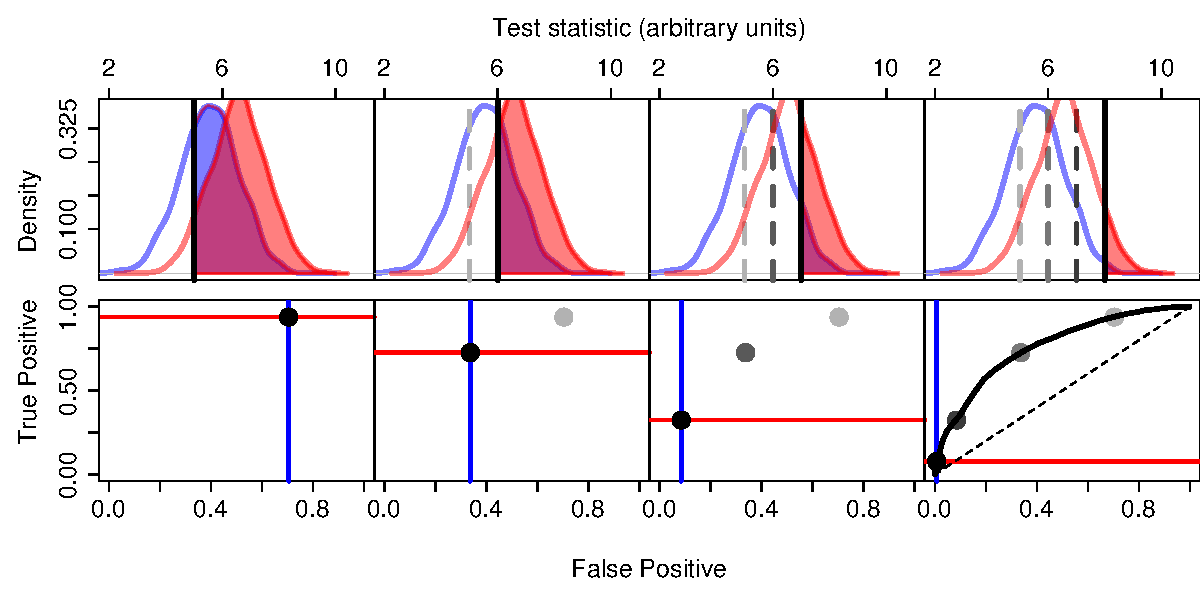
\includegraphics[width=\linewidth]{Fig1}
     \label{fig1}
     \caption{Top row: The distributions of a hypothetical warning indicator are shown under the case of a stable system (blue) and a system approaching a critical transition (red).  Bottom row: Points along the ROC curve are calculated for each possible threshold indicated in the top row.  The false positive rate is the integral of the distribution of the test statistic under the stable system right of the threshold (blue shaded area, corresponding to blue vertical line).  The true positive rate is the integral of the system approaching a transition left of the threshold (red shaded area, corresponds to the red line).  Successive columns show the threshold increasing, tracing out the ROC curve.}
  \end{center}
 \end{figure}



 \begin{figure}[h]
   \begin{center}
     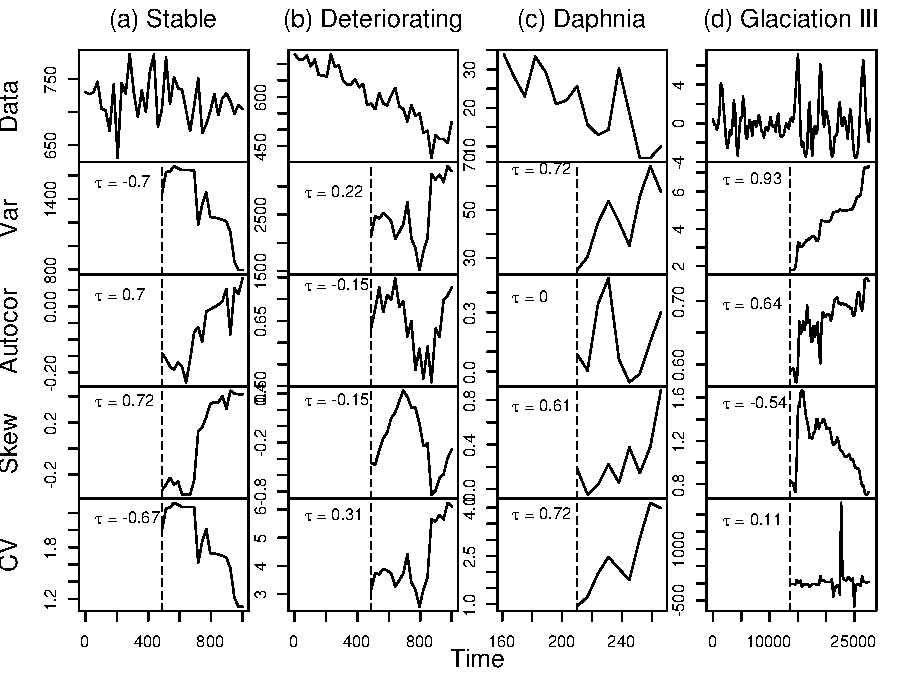
\includegraphics[width=\linewidth]{Fig2}
     \label{fig2}
     \caption{Early warning signals in simulated and empirical data sets.  The first two columns are simulated data from (a) a stable system (Stable), and (b) the same system approaching a saddle-node bifurcation (Deteriorating).  Empirical examples are from (c) \emph{Daphnia magna} concentrations manipulated towards a critical transition (Daphnia), and (d) deuterium concentrations previously cited as an early warning signal of a glaciation period (Glaciation). Increases in summary statistics, computed over a moving window, have often been used to indicate if a system is moving towards a critical transition.  The increase is measured by the correlation coefficient $\tau$.  Note that positive correlation does not guarantee the system is moving towards a transition, as seen in the stable system, first column.}
  \end{center}
 \end{figure}



 \begin{figure}[h]
   \begin{center}
     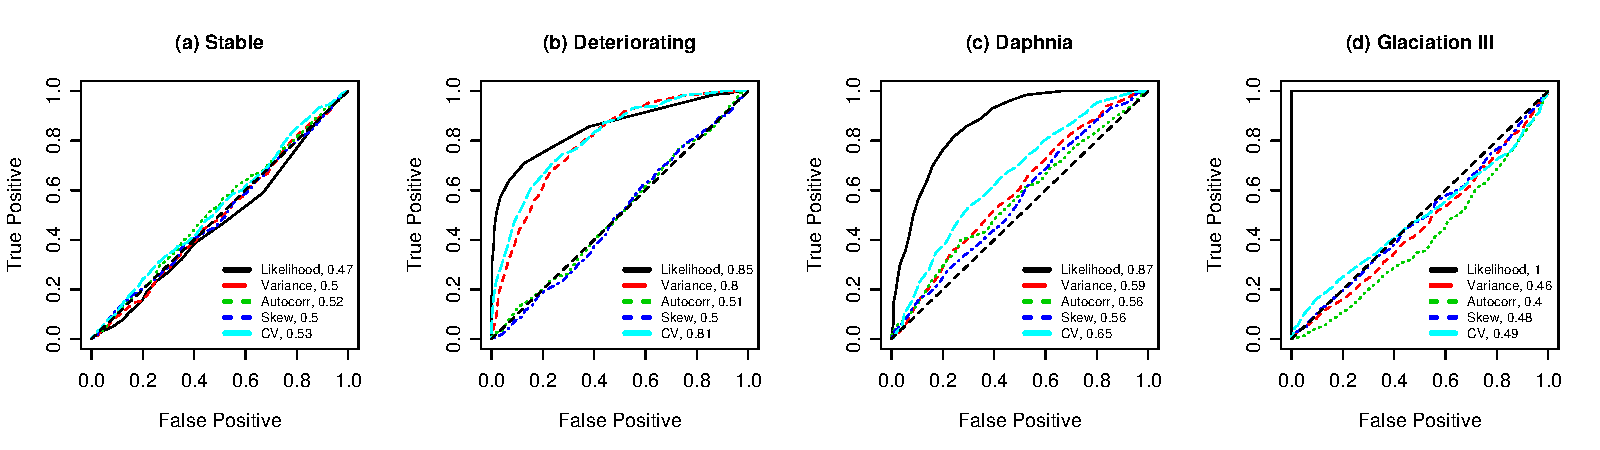
\includegraphics[width=\linewidth]{Fig3.pdf}
     \label{fig3}
     \caption{ROC curves for different early warning indicators on simulated and empirical data.  The area under the curve, inset, indicates how the method compares to a random guess (0.5).  The likelihood method performs substantially better than other metrics, particularly on the weaker trends seen in the empirical data. The simulated data sets have 40 points, ``Daphnia'' has 16, the ``Glaciation'' has 121. See corresponding distributions, Fig. S1.}
  \end{center}
 \end{figure}


 \begin{figure}[h!]
   \begin{center}
     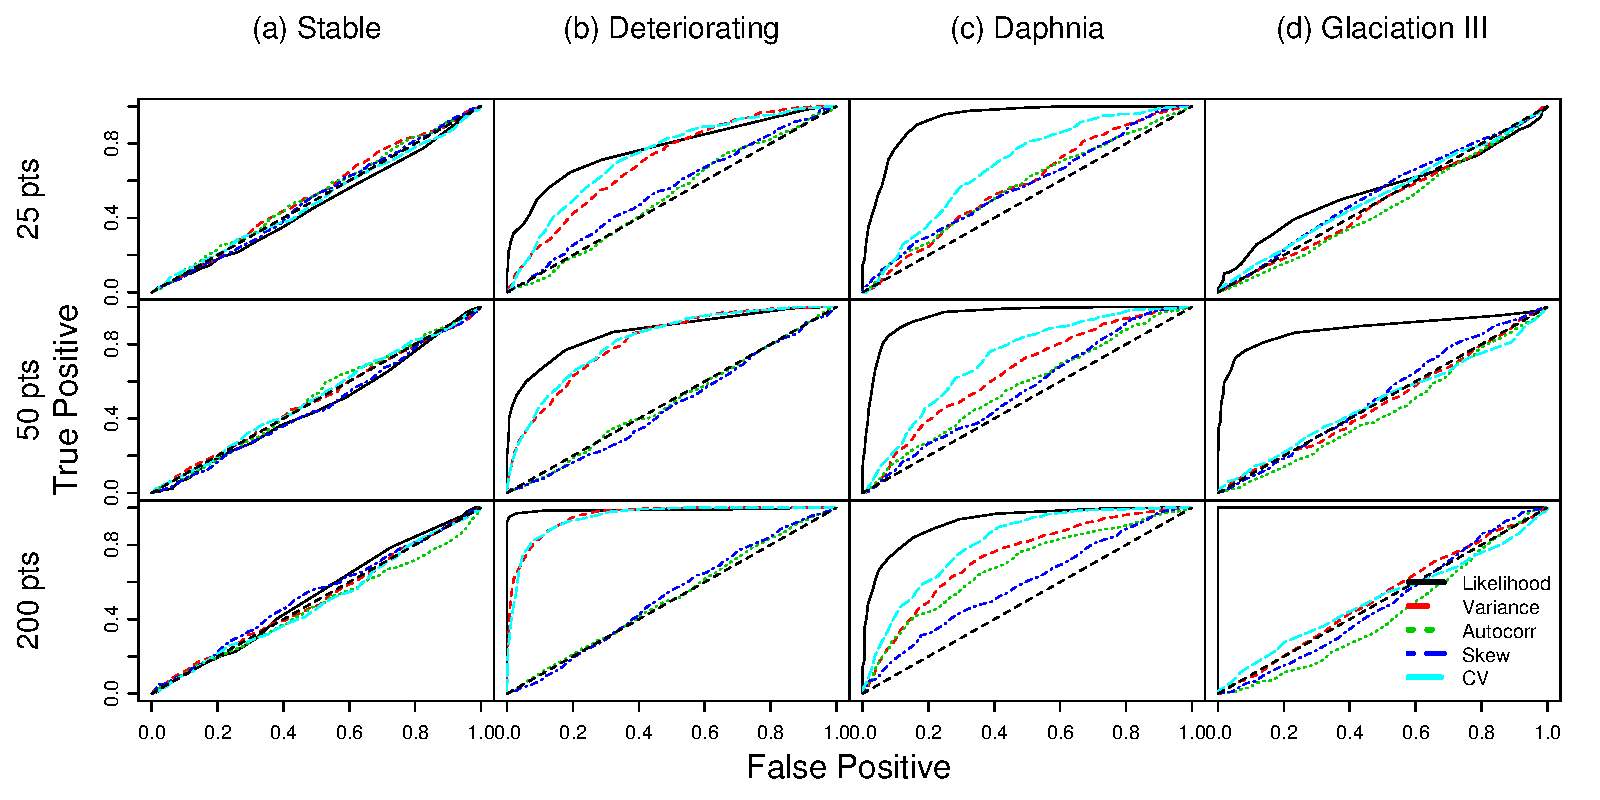
\includegraphics[width=\linewidth]{Fig4.pdf}
     \label{fig4}
     \caption{ROC curves (from Fig. 3) are recalculated under different sampling frequencies in the simulation step (see supplementary online text), using a total of 25, 50, or 200 points.  Increasing the sampling improves the trade-off between sensitivity and reliability for all indicators, though the likelihood approach is most effective. A warning signal is not detected in stable system simulation. Corresponding distributions shown in Fig S2-5.} 
  \end{center}
 \end{figure}

 \end{document}



